\section{Gestion de projet}
    \subsection{Réalisation d’un état des lieux du projet}

Afin de comprendre les sources du projet \COREL et le travail effectué lors des projets précédents, il a été nécessaire de faire un état des lieux, à intégrer dans le cahier des charges.\footnote{Voir l'annexe A} En effet, les projets \LSC et \EPJ n'ont pas produit de documentation, ce qui rend la compréhension de ces projets difficile. Seuls les chercheurs ayant travaillé sur ces projets sont à même d'expliquer le travail effectué et les productions qui en découlent. De plus, sans connaissances préalables sur le droit chinois, les sources numériques produites ne sont pas suffisamment claires pour être instantanément comprises par un ingénieur et ne se suffisent pas à elles-mêmes, d'autant plus avec un schéma d'encodage personnalisé, qui a pu se transformer avec le temps. Dès lors, l'état des lieux des projets précédents est indispensable afin de préparer les données pour le projet \COREL, d'autant plus que l'enrichissement des données \LSC et \EPJ est toujours en cours. 

En l'absence de documentation rédigée pendant le projet, ou de documents de travail détaillant les étapes de traitement des données effectuées, l'état des lieux fournit une description des sources numériques au début du projet \COREL. Puisque les sources \XML ont été transformées en \TEI pendant le stage, l'état des lieux n'est pas exhaustif sur le schéma d'encodage personnalisé du site \LSC mais fournit un aperçu de la transformation \XSLT et des raisons pour lesquelles le schéma \LSC ne convenait plus. Cette partie du cahier des charges vise à donner un premier aperçu des documents pour en comprendre la composition générale. 

Les productions du projet \EPJ sont, quant à elles, multiples et ont demandé une description plus approfondie. Appréhender ces données est un travail complexe, puisque les formats des données sont hétérogènes, même au sein du projet \EPJ. De plus, le travail étant effectué par un prestataire, l'équipe du projet n'a pas de visibilité sur les différentes étapes de travail effectuées pour aboutir à ces formats de données. L'état des lieux rédigé dans le cahier des charges reste donc une description des données fournies par le prestataire et du travail effectué par les chercheurs, mais ne peut détailler de manière exhaustive toutes les étapes de la chaîne de traitement.

L'état des lieux est organisé selon le type de données : les annotations, les métadonnées et les liens entre les lois. Ces trois types de données ne correspondent pas nécessairement à un seul format, c'est pourquoi organiser l'état des lieux un format après l'autre n'est pas pertinent et complexifie la compréhension. Les annotations, par exemple, sont accessibles au format \JSON, \csv ou \tsv et directement via le visualiseur Mirador. Ce travail de description s'accompagne parfois de modélisations \UML pour faciliter la compréhension. En effet, le recensement de tous les liens entre les lois est un fichier assez dense et complexe et qui ne possède pas de documentation. Seuls les chercheurs du projet \EPJ sont capables d'utiliser ce recensement comme outil de travail. Or, retracer la généalogie des lois est l'un des axes majeurs du projet, ce document est donc essentiel afin de réaliser le projet. Cet exemple permet de souligner l'importance de fournir une documentation et des documents de travail clairs. En effet, deux modélisations suffisent pour expliciter ce document et permettent de comprendre facilement quels types de liens sont possibles entre les lois. L'établissement d'un cahier des charges et la production d'une documentation pendant le stage sont donc essentiels pour la suite du projet.  

\begin{figure}
    \centering
    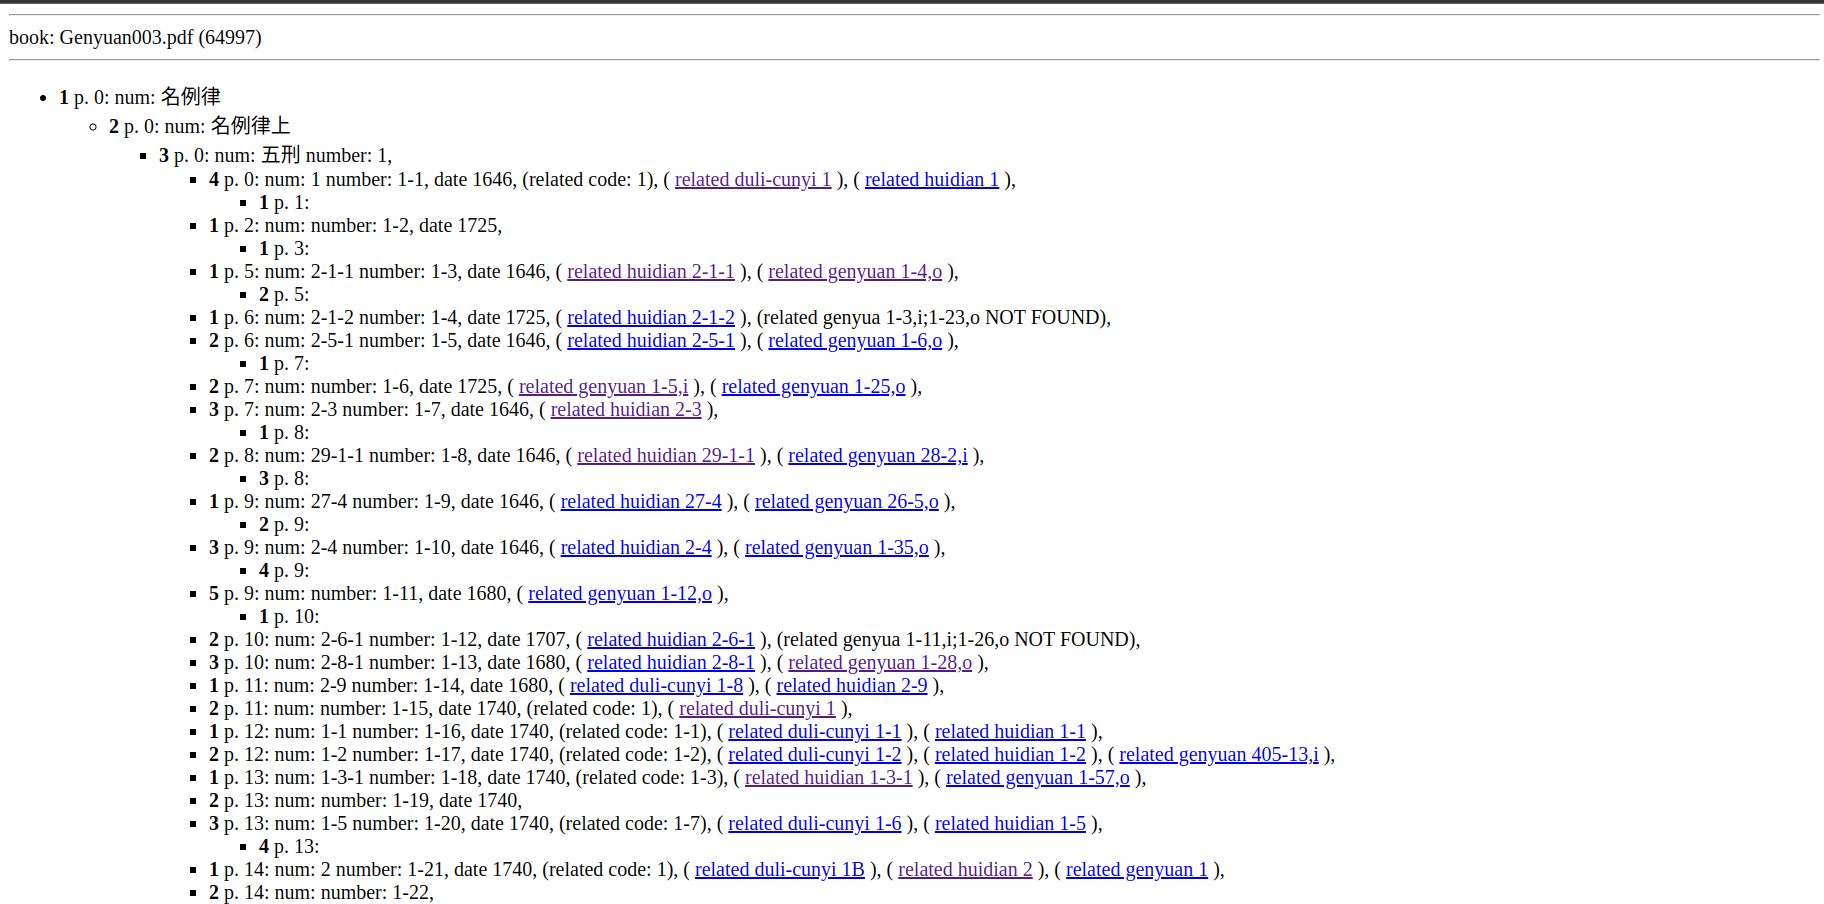
\includegraphics[width=\textwidth]{images/image6.png}
    \caption{Capture d'écran du fichier de recensement des liens entre les lois.}
\end{figure}

\subsection{Définir les livrables attendus du projet}

L'établissement d'un cahier des charges fonctionnel permet également de définir clairement les livrables attendus. Le projet \COREL n'avait jusqu'alors pas de descriptif précis des livrables attendus en fin de projet. Lors de la candidature à l'appel à projets pour le financement \CollEx Persée, les chercheurs ont défini comme livrable un \POC sur trois lois représentatives du corpus pour créer un \cv. Toutefois, ce livrable est considéré par l'équipe du projet comme un engagement minimal, et le périmètre du projet est en réalité plus large. 

Une grande partie du stage a donc été consacrée à définir ce périmètre, en assurant la cohésion entre le projet de recherche et sa réalisation technique, en prenant en considération la volonté des chercheurs d'élargir leur champ de compétences en participant à certains aspects numériques du projet, comme l'encodage par exemple. Il a donc fallu dans un premier temps rassembler les idées de chaque membre de l'équipe lors de réunions, tout en gardant à l'esprit le besoin d'utiliser des outils et méthodes accessibles aux chercheurs, c'est-à-dire sans pré-requis techniques. Lors des réunions de conception du projet, il s'est avéré que les chercheurs souhaitaient un livrable bien plus étendu que le \POC : une édition en ligne la plus exhaustive possible (ajout de commentaires, entités nommées...), la reconstitution de la législation entre 1644 et 1911 et également des visualisations interactives pour retracer la généalogie d'une loi. Ces livrables n'avaient toutefois pas été clairement définis car il était important pour l'équipe de rester flexible durant toute la durée du projet. Toutefois, cette manière d'envisager le projet présente un risque conséquent. En effet, sans livrable défini ni périmètre, le projet peut ne pas être réalisé dans le temps imparti du financement et laissé à l'abandon comme c'est le cas du site web \LSC. Le cahier des charges fonctionnels a ainsi permis aux chercheurs d'exprimer toutes leurs attentes et de fixer clairement le périmètre, en dialogue avec l'ingénieur du projet. 

\subsection{Prioriser certains aspects du projet}

Ce travail de définition des besoins et des livrables en sortie du projet ne signifie pas pour autant que le projet manque de flexibilité et lors des réunions, il est clairement apparu que les besoins du projet étaient hiérarchisés. En effet, une édition en ligne simple et la reconstitution de la législation sont les deux éléments les plus importants pour assurer la bonne réalisation du projet. Toutefois, le cahier des charges ne se limite pas à ces deux aspects du projet afin d'englober à la fois les besoins secondaires comme le balisage des entités nommées ou les visualisations, mais aussi les perspectives d'enrichissement futures. Trois niveaux du livrable final ont donc ainsi été définis : en premier lieu, tous les besoins hors périmètre ont été écartés du projet. Cela concerne les données dont le projet ne dispose pas, notamment les recueils de cas qui sont actuellement en cours de numérisation par la bibliothèque d'études chinoises. Ces données sont intéressantes du point de vue scientifique et apportent une plus-value aux textes de lois, mais ne sont pas indispensables dans le cadre du projet. Elles feront l'objet d'un autre projet ou seront ajoutées après l'échéance du financement. 

Il a ensuite fallu déterminer quelles données étaient primordiales pour la réalisation de l'édition en ligne et le \cv, et lesquelles seraient intéressantes à ajouter si le temps le permet. Le site \LSC permet de démontrer que les données en l'état sont suffisantes pour publier une édition en ligne. Toutefois, les données nécessaires au \cv ne figurent que dans les annotations et ne sont pas exhaustives. La priorité est donc d'ajouter ces données manquantes dans l'encodage \TEI, notamment les dates de validité de chaque loi et des identifiants uniques permettant de les lier aux annotations. Les ajouts de commentaires ou d'entités nommées, quant à eux, sont des éléments secondaires, mais qui font partie du périmètre car ils concernent les textes de lois déjà édités, et qu'une partie de ces données a déjà été balisée dans le \XML. 

Déterminer clairement les livrables attendus en priorisant certains aspects du projet a ainsi permis de lancer la phase de préparation des données sans écarter la possibilité de poursuivre le projet après le financement : les perspectives d'enrichissement sont détaillées dans des documents de travail clairs, qui permettront aux chercheurs ou aux ingénieurs de venir enrichir les données avec ces informations supplémentaires ultérieurement.

 \section{Importance de l’étape de préparation des données}
    \subsection{La diversité des données des projets précédents}

Une fois les données essentielles identifiées, il est possible de commencer à préparer les données. Cette étape est primordiale afin de réaliser le projet. En effet, lors du stage, la perspective de réaliser le \POC a été évoquée, mais a été écartée des missions de stage assez rapidement, car trop de données étaient manquantes. La priorité a donc été donnée au nettoyage, à l'adaptation et à la complétion des données. 

\subsubsection{Nettoyage des données}
La première partie du travail a permis de décider, en accord avec les chercheurs, quelles données issues des projets précédents étaient inutiles pour le projet \COREL. Le nettoyage des données consiste à corriger les données, notamment les erreurs. Toutefois, dans notre cas de figure, il est important de marquer une rupture entre les données des projets antérieurs et les données du projet \COREL. Dès lors, le nettoyage des données a essentiellement consisté à supprimer les données superflues, qui n'apportent aucune valeur ajoutée aux documents. Le travail de correction des erreurs, quant à lui, a été effectué par des employés du \cdf, car il est indispensable de lire le chinois pour cette tâche. Il est donc possible de considérer deux phases distinctes du nettoyage des données : le travail de correction de l'OCR et le travail de \og correction \fg de l'encodage et de tri des informations.

L'étape de nettoyage s'est donc effectuée tout au long du stage, en supprimant petit à petit les aspects de l'encodage qui ne servaient pas les objectifs du projet. En effet, dans un souci d'exhaustivité, l'équipe du projet souhaitait conserver un maximum d'informations dans l'encodage, afin de pouvoir réutiliser les sources pour d'autres types de projets par exemple. Cette problématique est récurrente dans les projets d'édition scientifique numérique, car le numérique offre des possibilités plus larges que le support papier, lequel contraint forcément l'éditeur à restreindre la volumétrie de son édition : 

\begin{quote}
    L’édition numérique permet de donner un grand nombre
d’informations à propos du texte. Si, dans le cadre de l’édition
papier, l’éditrice ou l’éditeur est souvent obligé de choisir
entre une approche méthodologique et une autre, le texte
numérique permet, quant à lui, de multiplier les données et de
proposer aussi des lectures et des interprétations parallèles.
Cependant il ne faut pas tomber dans le piège d’une sorte
d’idéologie d’exhaustivité. \footnote{\cite{vitali_rosati_les_2023}}
\end{quote}

Ainsi, malgré l'exhaustivité permise par le numérique, il était important de nettoyer les données issues des projets précédents pour ne pas tomber dans ce \og piège \fg et éviter les écueils qu'a déjà connu, notamment, le projet \LSC, vaste entreprise qui n'a pas été achevée. 

\subsubsection{Adaptation des données}
Les étapes de nettoyage et d'adaptation des données se sont déroulées en parallèle l'une de l'autre. En effet, le nettoyage des données fait partie du travail d'adaptation des données au projet \COREL, qui consiste à rendre les données non seulement exploitables pour le projet, mais surtout \textit{pensées} pour lui. La différence entre ces deux états des données est notamment démontrée par l'étape de nettoyage : dans les faits, laisser les balises de traduction anglaise et française du schéma \LSC n'est pas bloquant pour le projet. C'est d'ailleurs d'après ce postulat qu'a démarré la phase de préparation des données. Toutefois, outre la problématique d'exhaustivité, soulevée dans le point précédent, ces données supplémentaires n'apportent aucune plus-value à l'encodage, d'autant plus qu'elles sont pour la plupart vides, représentées par des balises auto-fermantes : \texttt{<content lang='fr'/>}. Ignorer ces ajouts n'est pas impossible en soit, mais pose deux soucis majeurs : le premier, purement pratique, est qu'inclure ces données inutiles dans l'encodage \XML ralentit le processus de préparation des données. En effet, les données \XML ont été transformées en \TEI, notamment pour que le schéma d'encodage devienne interopérable. Dès lors, ignorer ces balises superflues est impossible, puisque cela reviendrait à produire un document non valide, qui ne respecte pas le standard de la \TEI. Dans le cadre du projet, deux solutions ont été considérées : adapter, c'est-à-dire transformer ces balises selon les standards de la \TEI, ou bien nettoyer, c'est-à-dire dans ce cas de figure, les supprimer de l'encodage. La limite de temps et de financement sont des contraintes majeures de nombreux projets : dès lors, il est nécessaire d'adapter le périmètre. Ajouter des étapes supplémentaires de préparation des données n'était donc pas pertinent dans cette situation. L'exemple des balises de traduction est également représentatif du deuxième problème que soulève ce type de données superflues : la question des données propres (ou \textit{tidy data}). En effet, bien que les corrections de l'\OCR contribuent à rendre les données propres, un encodage verbeux, où toutes les balises sont triples pour envisager une édition trilingue qui ne fait partie ni du périmètre du projet, ni des perspectives d'enrichissement, rendent le code difficilement compréhensible. Plutôt que de servir le projet, ces balises le desservent, c'est pourquoi le nettoyage des données a en réalité consisté en l'extraction des données utiles au projet, en laissant de côté les informations spécifiques au projet \LSC.  


\subsection{Établissement d’un écosystème de données}

Le corpus étant encodé en \XML et en envisageant la perspective de publier les données via la plateforme \tp, le choix de données 100\% \XML pour le projet semble pertinent. Ainsi, il a été décidé d'ajouter les données extraites des fichiers \JSON dans l'encodage. Cette solution permet également d'utiliser uniquement la base de données \XML comme source de données, ce qui facilite la gestion des sources et ne demande pas de lier deux sources de données différentes. Cela est réalisable pour produire deux aspects du site web : l'édition en ligne et la reconstitution de la législation (le \cv). Cependant, une fois les livrables clairement définis, cette solution ne s'est pas révélée pleinement satisfaisante, notamment pour réaliser les visualisations. En effet, bien que cette partie du projet ne soit pas prioritaire, elle entre tout de même dans le périmètre et doit être prise en considération. Afin de réaliser des visualisations interactives, la solution la plus courante est de recourir au \JS. Dès lors, conserver les fichiers \JSON et les lier aux sources \XML s'est avéré plus pertinent pour cet aspect du projet. 

Une solution hybride a donc été choisie afin de faciliter la réalisation de chaque partie du livrable. Les données nécessaires à édition en ligne ainsi qu'au \cv seront contenues dans le \XML, tandis que les données relatives à la généalogie des lois, déjà présentes dans le \JSON, permettront de réaliser les visualisations. En effet, tout comme transformer les données des anciens projets demandaient des étapes de traitement des données supplémentaires, implémenter les données des liens entre les lois représentait un travail fastidieux en plus d'être injustifié, puisque le recours au langage \JS privilégie le format \JSON. 

Dès lors, l'établissement d'un écosystème de données, afin de lier deux formats de données différents, a été nécessaire. Une fois les données des fichiers \JSON complétées par le prestataire, des identifiants permettront de lier chaque loi à son annotation. L'intérêt d'ajouter des identifiants est double : cela permet non seulement de lier les deux sources de données entre elles, mais également de permettre le dédoublonnage des lois lors de la réalisation du \cv, puisque certaines lois apparaissent dans plusieurs textes. Considérer l'encodage \XML comme source de données principale, et la lier aux annotations comme sources de données secondaires, est donc l'architecture de données la plus appropriée au projet \COREL. 
